% ===================================================================
%  Week 2 — Session 1: Histograms & Point Operations
%  Compile: pdflatex -interaction=nonstopmode slides-a.tex  (twice)
% ===================================================================
\documentclass[10pt,aspectratio=169]{beamer}
% ===================================================================
%  Shared Beamer preamble for "Practical Image Processing"
%  English slides. Compile with pdfLaTeX.
% ===================================================================

\usetheme{metropolis}
\usepackage[T1]{fontenc}
\usepackage[utf8]{inputenc}
\usepackage{lmodern}
\usepackage{listings}
\usepackage{tcolorbox}
\usepackage{fontawesome5}
\usepackage{booktabs}
\usepackage{amsmath,amssymb}
\usepackage{tikz}
\usepackage{pgfplots}
\pgfplotsset{compat=1.17}
\usetikzlibrary{arrows.meta,positioning,shapes.geometric,fit,backgrounds,matrix}
\tcbuselibrary{skins,breakable}

% ---- Palette --------------------------------------------------------
\definecolor{coursePrimary}{HTML}{1B4965}   % deep blue
\definecolor{courseAccent}{HTML}{E76F51}    % coral
\definecolor{courseGood}{HTML}{2A9D8F}      % teal
\definecolor{courseBad}{HTML}{C0392B}       % red
\definecolor{courseInfo}{HTML}{2980B9}      % blue
\definecolor{codeBg}{HTML}{F5F6FA}
\definecolor{codeKw}{HTML}{8E44AD}
\definecolor{codeStr}{HTML}{2A9D8F}
\definecolor{codeCom}{HTML}{7F8C8D}

\setbeamercolor{frametitle}{bg=coursePrimary}
\setbeamercolor{progress bar}{fg=courseAccent}
\setbeamercolor{alerted text}{fg=courseAccent}
\metroset{block=fill,sectionpage=progressbar,numbering=fraction}

% ---- Code listings (Python is built into listings) -----------------
\lstdefinestyle{course}{
  backgroundcolor=\color{codeBg},
  basicstyle=\ttfamily\scriptsize,
  keywordstyle=\color{codeKw}\bfseries,
  stringstyle=\color{codeStr},
  commentstyle=\color{codeCom}\itshape,
  numberstyle=\tiny\color{codeCom},
  numbers=left, numbersep=6pt,
  showstringspaces=false, breaklines=true, breakatwhitespace=true,
  tabsize=4, columns=fullflexible,
  frame=single, framesep=4pt, rulecolor=\color{gray!30},
  keepspaces=true, upquote=true, language=Python,
}
\lstset{style=course}
\lstdefinelanguage{bash}{
  keywords={cd,pip,python,venv,source,import}, sensitive=true,
  morecomment=[l]{\#}, morestring=[b]', morestring=[b]",
}

% ---- Reusable callout boxes ----------------------------------------
\newtcolorbox{goodbox}[1][Good practice]{colback=courseGood!8,colframe=courseGood,
  fonttitle=\bfseries,title={\faCheck~#1},boxrule=0.6pt,left=4pt,right=4pt,top=3pt,bottom=3pt}
\newtcolorbox{badbox}[1][Pitfall]{colback=courseBad!8,colframe=courseBad,
  fonttitle=\bfseries,title={\faTimes~#1},boxrule=0.6pt,left=4pt,right=4pt,top=3pt,bottom=3pt}
\newtcolorbox{infobox}[1][Note]{colback=courseInfo!8,colframe=courseInfo,
  fonttitle=\bfseries,title={\faInfoCircle~#1},boxrule=0.6pt,left=4pt,right=4pt,top=3pt,bottom=3pt}
\newtcolorbox{mathbox}[1][Math]{colback=coursePrimary!6,colframe=coursePrimary,
  fonttitle=\bfseries,title={\faCalculator~#1},boxrule=0.6pt,left=4pt,right=4pt,top=3pt,bottom=3pt}

\newcommand{\keyidea}[1]{\begin{alertblock}{Key idea}#1\end{alertblock}}
\newcommand{\term}[1]{\textbf{\color{coursePrimary}#1}}
\newcommand{\code}[1]{\lstinline[basicstyle=\ttfamily\small]|#1|}

% ---- A helper to draw a small pixel grid, cells shaded by value ----
% \pixelgrid{ {10,20,120,200,240}, {30,60,130,180,230}, ... }
\newcommand{\pixelgrid}[1]{%
  \begin{tikzpicture}[font=\scriptsize,scale=0.6]
    \foreach \row [count=\ry] in {#1} {
      \foreach \val [count=\cx] in \row {
        \draw[gray,fill=coursePrimary!8] (\cx,-\ry) rectangle ++(1,-1);
        \node at (\cx+0.5,-\ry-0.5) {\val};
      }
    }
  \end{tikzpicture}}


\title{Point Operations \& Histograms}
\subtitle{Week 2 — Session 1: Reading the histogram \& per-pixel fixes}
\author{Practical Image Processing}
\date{Lecture 2.1 \textbullet\ 60--70 min}

\begin{document}

\maketitle

\begin{frame}{Recap \& today}
  \begin{columns}[T]
    \begin{column}{0.58\textwidth}
      \begin{itemize}
        \item Wk1: an image is numbers on a grid; watch BGR, uint8, and \code{[y,x]} indexing.
        \item \alert{Today (Session 1):} the \term{histogram} — the tool that tells you what a
              transform should do — and \term{point operations} that transform each pixel by itself.
        \item Session 2 will build on this for \term{thresholding} and advanced enhancement.
      \end{itemize}
    \end{column}
    \begin{column}{0.42\textwidth}
      \begin{alertblock}{Why it matters}
        DocScan's meter photos are often too dark or low-contrast. Fixing exposure is step one
        to reading the digits.
      \end{alertblock}
    \end{column}
  \end{columns}
\end{frame}

\begin{frame}{Roadmap}\tableofcontents\end{frame}

% ==================================================================
\section{The histogram}
% ==================================================================

\begin{frame}{The histogram: a census of brightness}
  \begin{columns}[T]
    \begin{column}{0.5\textwidth}
      A real meter crop and its histogram:
      \begin{center}
      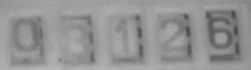
\includegraphics[width=\linewidth]{../assets/gray.png}\\[3pt]
      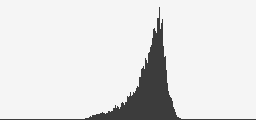
\includegraphics[width=\linewidth]{../assets/hist_before.png}
      \end{center}
    \end{column}
    \begin{column}{0.5\textwidth}
      \begin{itemize}
        \item $x$-axis: intensity 0--255. $y$-axis: how many pixels have it.
        \item This histogram is bunched $\rightarrow$ \term{low contrast} (digits barely stand out).
        \item Read the histogram \emph{before} touching the image.
      \end{itemize}
      \begin{infobox}[Definition]
        For a gray image, $h(k)$ = number of pixels with intensity $k$, for $k=0,\dots,255$.
      \end{infobox}
    \end{column}
  \end{columns}
\end{frame}

\begin{frame}{Reading a histogram}
  \begin{center}
  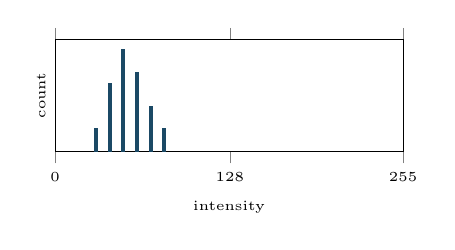
\begin{tikzpicture}
    \begin{axis}[width=6cm,height=3cm,ybar,bar width=1pt,ymin=0,xmin=0,xmax=255,
      xtick={0,128,255},ytick=\empty,font=\tiny,xlabel={intensity},ylabel={count}]
      \addplot[draw=coursePrimary,fill=coursePrimary] coordinates{(30,2)(40,6)(50,9)(60,7)(70,4)(80,2)};
    \end{axis}
  \end{tikzpicture}
  \end{center}
  \begin{itemize}
    \item Peak on the \term{left} = dark (under-exposed). On the \term{right} = bright.
    \item \term{Narrow} = low contrast. \term{Spread across the range} = good contrast.
    \item Two peaks (\term{bimodal}) = object vs background — a gift for thresholding (Session 2).
  \end{itemize}
\end{frame}

\begin{frame}{Four histogram shapes you must recognise}
  \begin{columns}[T]
    \begin{column}{0.5\textwidth}\begin{center}
      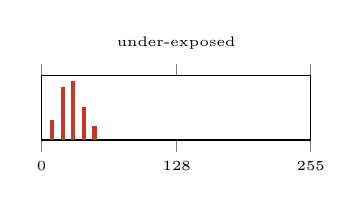
\begin{tikzpicture}
        \begin{axis}[width=5cm,height=2.4cm,ybar,bar width=1.2pt,ymin=0,xmin=0,xmax=255,
          xtick={0,128,255},ytick=\empty,font=\tiny,title={\tiny under-exposed}]
          \addplot[draw=courseBad,fill=courseBad] coordinates{(10,3)(20,8)(30,9)(40,5)(50,2)};
        \end{axis}
      \end{tikzpicture}\\
      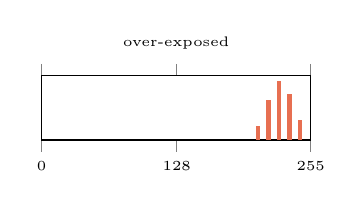
\begin{tikzpicture}
        \begin{axis}[width=5cm,height=2.4cm,ybar,bar width=1.2pt,ymin=0,xmin=0,xmax=255,
          xtick={0,128,255},ytick=\empty,font=\tiny,title={\tiny over-exposed}]
          \addplot[draw=courseAccent,fill=courseAccent] coordinates{(205,2)(215,6)(225,9)(235,7)(245,3)};
        \end{axis}
      \end{tikzpicture}
    \end{center}\end{column}
    \begin{column}{0.5\textwidth}\begin{center}
      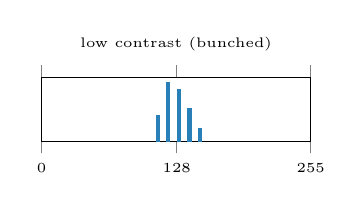
\begin{tikzpicture}
        \begin{axis}[width=5cm,height=2.4cm,ybar,bar width=1.2pt,ymin=0,xmin=0,xmax=255,
          xtick={0,128,255},ytick=\empty,font=\tiny,title={\tiny low contrast (bunched)}]
          \addplot[draw=courseInfo,fill=courseInfo] coordinates{(110,4)(120,9)(130,8)(140,5)(150,2)};
        \end{axis}
      \end{tikzpicture}\\
      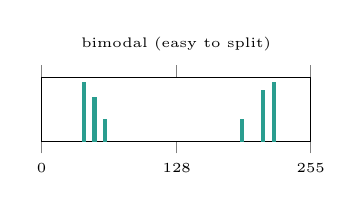
\begin{tikzpicture}
        \begin{axis}[width=5cm,height=2.4cm,ybar,bar width=1.2pt,ymin=0,xmin=0,xmax=255,
          xtick={0,128,255},ytick=\empty,font=\tiny,title={\tiny bimodal (easy to split)}]
          \addplot[draw=courseGood,fill=courseGood] coordinates{(40,8)(50,6)(60,3)(190,3)(210,7)(220,8)};
        \end{axis}
      \end{tikzpicture}
    \end{center}\end{column}
  \end{columns}
  \vspace{2pt}
  \keyidea{Diagnose the shape first — it decides \emph{whether} and \emph{which} enhancement to apply.}
\end{frame}

\begin{frame}[fragile]{Computing a histogram}
\begin{lstlisting}[language=Python]
import cv2, numpy as np
gray = cv2.cvtColor(cv2.imread('E:/data/abfa_image/numerators/num_3494.jpg'),
                    cv2.COLOR_BGR2GRAY)
hist = cv2.calcHist([gray], [0], None, [256], [0, 256])  # 256 bins
print(gray.min(), gray.max(), gray.mean())   # quick exposure check
\end{lstlisting}
  \keyidea{The histogram throws away \emph{where} pixels are and keeps \emph{how many} of each value.
  That's exactly what you need to reason about exposure and contrast.}
\end{frame}

\begin{frame}{Worked example: histogram of a tiny image}
  \begin{columns}[T]
    \begin{column}{0.42\textwidth}
      A $4\times4$ patch of intensities:
      \begin{center}
      \pixelgrid{ {10,10,40,40}, {10,20,40,60}, {20,20,60,60}, {20,40,60,90} }
      \end{center}
    \end{column}
    \begin{column}{0.58\textwidth}
      Tally each value:
      \begin{center}\footnotesize
      \begin{tabular}{lcccccc}
        \toprule
        value $k$ & 10 & 20 & 40 & 60 & 90 \\
        \midrule
        count $h(k)$ & 3 & 4 & 4 & 4 & 1 \\
        \bottomrule
      \end{tabular}
      \end{center}
      \begin{itemize}
        \item 16 pixels total; range is only $[10,90]$ — nothing near white.
        \item Bunched \& dark $\rightarrow$ a stretch or gamma will help.
      \end{itemize}
    \end{column}
  \end{columns}
\end{frame}

% ==================================================================
\section{Point operations}
% ==================================================================

\begin{frame}{Point operations: one pixel at a time}
  \begin{itemize}
    \item A \term{point operation} maps each pixel's value through a function $s = T(r)$ — independent of neighbours.
    \item Brightness: $s = r + b$. Contrast: $s = a\cdot r$. Negative: $s = 255 - r$.
    \item Implemented as a \term{lookup table} (LUT): compute $T$ once for 0--255, apply to all pixels fast.
  \end{itemize}
  \begin{mathbox}
    General linear: $s = a\cdot r + b$ — $a$ scales contrast, $b$ shifts brightness. Then clip to 0--255.
  \end{mathbox}
\end{frame}

\begin{frame}{The LUT: compute once, apply everywhere}
  \begin{center}
  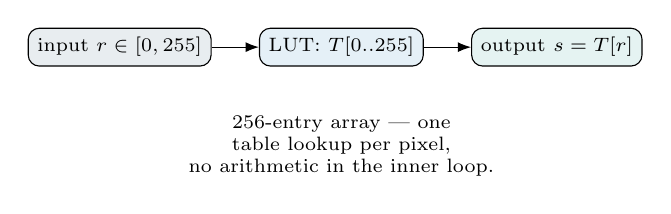
\begin{tikzpicture}[font=\scriptsize,node distance=6mm]
    \node[draw,rounded corners,fill=coursePrimary!10] (r) {input $r\in[0,255]$};
    \node[draw,rounded corners,fill=courseInfo!12,right=of r] (t) {LUT: $T[0..255]$};
    \node[draw,rounded corners,fill=courseGood!12,right=of t] (s) {output $s=T[r]$};
    \draw[-{Latex}] (r)--(t);
    \draw[-{Latex}] (t)--(s);
    \node[below=5mm of t,align=center,text width=5.2cm]
      {256-entry array — one table lookup per pixel,\\ no arithmetic in the inner loop.};
  \end{tikzpicture}
  \end{center}
  \begin{itemize}
    \item Any per-pixel function (linear, gamma, negative, threshold) is \emph{just a different table}.
    \item Cost is independent of image size in the table build; application is one pass, $O(N)$.
  \end{itemize}
\end{frame}

\begin{frame}{The transfer function $s=T(r)$}
  \begin{columns}[T]
    \begin{column}{0.55\textwidth}
    \begin{center}
    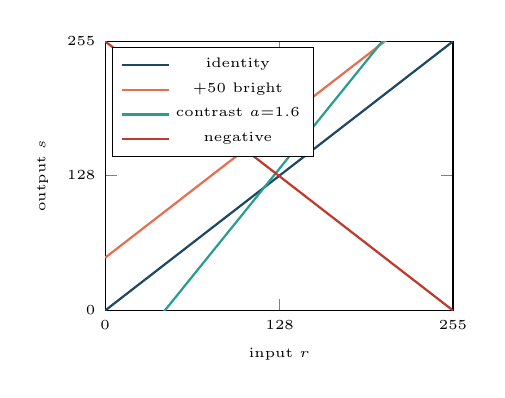
\begin{tikzpicture}
      \begin{axis}[width=6cm,height=5cm,xmin=0,xmax=255,ymin=0,ymax=255,font=\tiny,
        xlabel={input $r$},ylabel={output $s$},legend style={font=\tiny,at={(0.02,0.98)},anchor=north west},
        xtick={0,128,255},ytick={0,128,255}]
        \addplot[coursePrimary,thick,domain=0:255,samples=2]{x};\addlegendentry{identity}
        \addplot[courseAccent,thick,domain=0:255,samples=2]{x+50};\addlegendentry{$+50$ bright}
        \addplot[courseGood,thick,domain=0:255,samples=2]{1.6*x-70};\addlegendentry{contrast $a{=}1.6$}
        \addplot[courseBad,thick,domain=0:255,samples=2]{255-x};\addlegendentry{negative}
      \end{axis}
    \end{tikzpicture}
    \end{center}
    \end{column}
    \begin{column}{0.45\textwidth}
      \begin{itemize}
        \item The \term{shape} of $T$ is the whole story.
        \item Slope $=$ contrast; vertical offset $=$ brightness.
        \item Anything above 255 or below 0 is \term{clipped} (flat ends of the real curve).
      \end{itemize}
    \end{column}
  \end{columns}
\end{frame}

\begin{frame}{Worked example: a linear map with clipping}
  \begin{mathbox}
    $s = \mathrm{clip}(a\,r + b,\,0,\,255)$ with $a=1.5,\ b=-40$.
  \end{mathbox}
  \begin{center}\footnotesize
  \begin{tabular}{lccccc}
    \toprule
    $r$ & 20 & 60 & 120 & 200 & 240 \\
    $a r + b$ & $-10$ & 50 & 140 & 260 & 320 \\
    $s$ (clipped) & \textbf{0} & 50 & 140 & \textbf{255} & \textbf{255} \\
    \bottomrule
  \end{tabular}
  \end{center}
  \begin{itemize}
    \item Dark pixels ($r=20$) get crushed to 0; bright ones ($\geq 200$) saturate at 255.
    \item Contrast $a>1$ steepens the middle but \term{loses} detail at both ends.
  \end{itemize}
  \begin{badbox}
    Forgetting to clip (and letting uint8 wrap around) turns bright pixels black — a classic bug.
  \end{badbox}
\end{frame}

\begin{frame}{Gamma correction — on the real meter}
  \begin{columns}[T]
    \begin{column}{0.33\textwidth}\begin{center}
      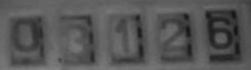
\includegraphics[width=\linewidth]{../assets/gamma_dark.png}\\{\scriptsize $\gamma<1$ (darker)}
    \end{center}\end{column}
    \begin{column}{0.33\textwidth}\begin{center}
      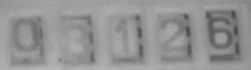
\includegraphics[width=\linewidth]{../assets/gray.png}\\{\scriptsize original}
    \end{center}\end{column}
    \begin{column}{0.33\textwidth}\begin{center}
      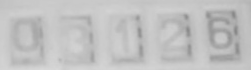
\includegraphics[width=\linewidth]{../assets/gamma_bright.png}\\{\scriptsize $\gamma>1$ (brighter)}
    \end{center}\end{column}
  \end{columns}
  \vspace{4pt}
  \begin{mathbox}
    $s = 255\,(r/255)^{1/\gamma}$ — a \emph{nonlinear} curve that brightens shadows without blowing out highlights.
  \end{mathbox}
\end{frame}

\begin{frame}{The gamma curve, drawn}
  \begin{columns}[T]
    \begin{column}{0.55\textwidth}
    \begin{center}
    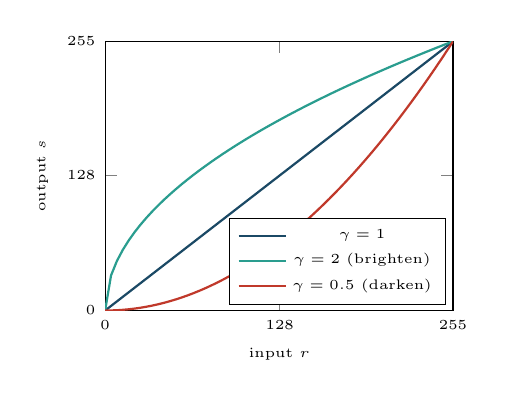
\begin{tikzpicture}
      \begin{axis}[width=6cm,height=5cm,xmin=0,xmax=255,ymin=0,ymax=255,font=\tiny,
        xlabel={input $r$},ylabel={output $s$},legend style={font=\tiny,at={(0.98,0.02)},anchor=south east},
        xtick={0,128,255},ytick={0,128,255},samples=60]
        \addplot[coursePrimary,thick,domain=0:255]{x};\addlegendentry{$\gamma=1$}
        \addplot[courseGood,thick,domain=0:255]{255*(x/255)^(0.5)};\addlegendentry{$\gamma=2$ (brighten)}
        \addplot[courseBad,thick,domain=0:255]{255*(x/255)^(2)};\addlegendentry{$\gamma=0.5$ (darken)}
      \end{axis}
    \end{tikzpicture}
    \end{center}
    \end{column}
    \begin{column}{0.45\textwidth}
      \begin{itemize}
        \item Curve \term{above} the diagonal lifts shadows (brightens); \term{below} darkens.
        \item Endpoints stay pinned at 0 and 255 — no clipping, unlike linear.
        \item The steep part near dark values is why gamma recovers hidden digits.
      \end{itemize}
    \end{column}
  \end{columns}
\end{frame}

\begin{frame}{Brightness/contrast vs gamma}
  \begin{itemize}
    \item Linear ($a r + b$) shifts/scales everything equally — can clip highlights or crush shadows.
    \item Gamma is \term{nonlinear}: it lifts dark tones more than bright ones (or vice versa).
    \item For a dark meter photo, gamma often recovers digits that a linear brighten would wash out.
  \end{itemize}
  \begin{goodbox}
    Match the tool to the histogram: shifted-but-spread $\rightarrow$ brightness; bunched $\rightarrow$ contrast/gamma.
  \end{goodbox}
\end{frame}

% ==================================================================
\section{Contrast enhancement}
% ==================================================================

\begin{frame}{Contrast stretching (min--max)}
  \begin{columns}[T]
    \begin{column}{0.55\textwidth}
      \begin{center}
      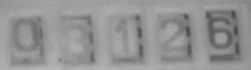
\includegraphics[width=0.9\linewidth]{../assets/gray.png}\\{\scriptsize before}\\[4pt]
      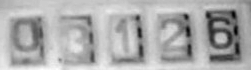
\includegraphics[width=0.9\linewidth]{../assets/stretch.png}\\{\scriptsize after: stretched to 0--255}
      \end{center}
    \end{column}
    \begin{column}{0.45\textwidth}
      \begin{itemize}
        \item Map the actual $[\min,\max]$ to the full $[0,255]$.
        \item Simple, reversible, and it can't invent detail — just uses the full range.
      \end{itemize}
      \begin{mathbox}
        $s = 255\dfrac{r-\min}{\max-\min}$
      \end{mathbox}
    \end{column}
  \end{columns}
\end{frame}

\begin{frame}{Worked example: stretching the tiny patch}
  \begin{mathbox}
    Patch range was $[\min,\max]=[10,90]$, so $s = 255\dfrac{r-10}{80}$.
  \end{mathbox}
  \begin{center}\footnotesize
  \begin{tabular}{lccccc}
    \toprule
    $r$ & 10 & 20 & 40 & 60 & 90 \\
    $s$ & 0 & 32 & 96 & 159 & 255 \\
    \bottomrule
  \end{tabular}
  \end{center}
  \begin{itemize}
    \item The darkest value goes to pure black, the brightest to pure white.
    \item Same \emph{ordering}, now spanning the full range — contrast is maximised without new detail.
  \end{itemize}
  \begin{badbox}
    A single bright speck (outlier max) can ruin a min--max stretch. Use \term{percentile} clipping (e.g. 2\%--98\%) instead.
  \end{badbox}
\end{frame}

\begin{frame}{Histogram equalization}
  \begin{columns}[T]
    \begin{column}{0.5\textwidth}
      \begin{center}
      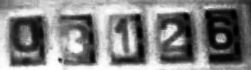
\includegraphics[width=0.85\linewidth]{../assets/equalized.png}\\{\scriptsize equalized meter}\\[3pt]
      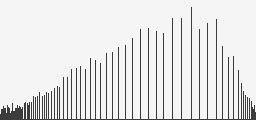
\includegraphics[width=0.85\linewidth]{../assets/hist_after.png}\\{\scriptsize its histogram — spread out}
      \end{center}
    \end{column}
    \begin{column}{0.5\textwidth}
      \begin{itemize}
        \item Redistributes intensities so the histogram is (roughly) \term{uniform}.
        \item Uses the \term{cumulative histogram} (CDF) as the mapping function.
        \item Great for revealing detail in low-contrast images — but can over-amplify noise.
      \end{itemize}
    \end{column}
  \end{columns}
\end{frame}

\begin{frame}{Equalization = use the CDF as the map}
  \begin{mathbox}
    $s = \mathrm{round}\!\left(255\cdot \mathrm{CDF}(r)\right)$, where $\mathrm{CDF}(r)=\dfrac{1}{N}\sum_{k\le r} h(k)$.
  \end{mathbox}
  \begin{itemize}
    \item The CDF is monotonic and rises fastest where pixels are \emph{crowded}.
    \item Crowded values get spread apart (more contrast there); empty ranges get compressed.
    \item Result: the output histogram is as flat as a discrete image allows.
  \end{itemize}
\end{frame}

\begin{frame}{Worked example: equalizing the tiny patch}
  \begin{center}\footnotesize
  \begin{tabular}{lccccc}
    \toprule
    $r$ & 10 & 20 & 40 & 60 & 90 \\
    $h(k)$ & 3 & 4 & 4 & 4 & 1 \\
    cumulative & 3 & 7 & 11 & 15 & 16 \\
    $\mathrm{CDF}=\text{cum}/16$ & 0.19 & 0.44 & 0.69 & 0.94 & 1.00 \\
    $s=255\,\mathrm{CDF}$ & 48 & 112 & 175 & 239 & 255 \\
    \bottomrule
  \end{tabular}
  \end{center}
  \begin{itemize}
    \item Five bunched dark values are pushed across the whole range.
    \item Notice the spacing follows the counts — dense region (10--60) fans out most.
  \end{itemize}
\end{frame}

\begin{frame}[fragile]{The three, in code}
\begin{lstlisting}[language=Python]
stretch = cv2.normalize(gray, None, 0, 255, cv2.NORM_MINMAX)
equalized = cv2.equalizeHist(gray)
lut = np.array([((i/255)**(1/0.5))*255 for i in range(256)], np.uint8)
gamma = cv2.LUT(gray, lut)                 # gamma = 0.5
\end{lstlisting}
  \begin{infobox}
    \code{cv2.LUT} applies a 256-entry table to every pixel in one fast pass — the pattern for any point op.
  \end{infobox}
\end{frame}

% ==================================================================
\section{In-class exercise}
% ==================================================================

\begin{frame}{\faPen~In-class exercise (10 min)}
  \begin{infobox}[Diagnose from the histogram]
  \end{infobox}
  You are handed three meter photos. Their histograms are:
  \begin{enumerate}
    \item a tall spike near 0, nothing above 80;
    \item two separated humps, one near 40 and one near 210;
    \item a smooth spread from 0 to 255.
  \end{enumerate}
  For each: is it under/over-exposed, low-contrast, or fine? Which operation would you apply,
  and which needs \emph{no} enhancement? Which one is easiest to threshold, and why?
\end{frame}

\begin{frame}{\faPen~Debrief}
  \begin{itemize}
    \item (1) Under-exposed \& low-contrast $\rightarrow$ gamma ($\gamma>1$) or stretch; digits hide in the dark.
    \item (2) Bimodal $\rightarrow$ already separable; \emph{ideal} for thresholding (object vs background).
    \item (3) Well-exposed, full range $\rightarrow$ leave it; enhancing may only amplify noise.
  \end{itemize}
  \keyidea{The histogram tells you \emph{whether} and \emph{which} enhancement — before you try anything.}
\end{frame}

% ==================================================================
\section{Wrap-up}
% ==================================================================

\begin{frame}{Pitfalls \& good practice}
  \begin{columns}[T]
    \begin{column}{0.5\textwidth}
      \begin{badbox}
        \begin{itemize}
          \item Not clipping $\rightarrow$ uint8 wrap-around (bright becomes black).
          \item Min--max stretch wrecked by one outlier pixel.
          \item Equalizing before you know the histogram shape.
        \end{itemize}
      \end{badbox}
    \end{column}
    \begin{column}{0.5\textwidth}
      \begin{goodbox}
        \begin{itemize}
          \item Print \code{min/max/mean} before choosing a fix.
          \item Prefer \term{deterministic} ops (gamma/stretch) in a pipeline.
          \item Build the LUT once; apply with \code{cv2.LUT}.
        \end{itemize}
      \end{goodbox}
    \end{column}
  \end{columns}
\end{frame}

\begin{frame}{What you should now be able to do}
  \begin{itemize}
    \item Read a histogram to diagnose exposure and contrast.
    \item Apply brightness, contrast, gamma, stretching, and equalization — and know which fits.
    \item Reason about a point operation as a transfer function $s=T(r)$ and a LUT.
    \item Hand-compute a stretch and an equalization on a small histogram.
  \end{itemize}
\end{frame}

\begin{frame}{Next session}
  \begin{alertblock}{Session 2 — Thresholding \& advanced enhancement}
    \begin{itemize}
      \item Turn a gray image into a clean digit \term{mask}: global (Otsu) vs \term{adaptive} thresholding.
      \item \term{CLAHE}, histogram matching, and enhancing \term{color} the right way (value channel).
      \item The full DocScan chain: enhance $\rightarrow$ threshold $\rightarrow$ clean.
    \end{itemize}
  \end{alertblock}
  \begin{center}\footnotesize Bring your histogram diagnoses from today — we act on them next time.\end{center}
\end{frame}

\begin{frame}[standout]
  Look at the histogram first.\\[4pt]
  \normalsize It tells you what the image needs before you change a single pixel.
\end{frame}

\end{document}
